\documentclass[12pt]{article} %Basic document type
\usepackage{times} %Font 
\usepackage{amsmath} %For matrices
\usepackage{amssymb}
\usepackage[section]{placeins} %Allows FloatBarrier command
\usepackage[utf8]{inputenc} %Font encoding
\usepackage[margin=1.25in]{geometry} %Adjust margins
\usepackage{graphicx} %Allows picture import
\usepackage{pdfpages} %Including pdf files 
\usepackage{setspace}
\usepackage{fancyhdr}
\usepackage{appendix}
\graphicspath{{images/}} %Allows picture impor
\pagestyle{fancy}
\fancyhf{}
\fancyhead[L]{The Inverted Pendulum}
\fancyhead[R]{ECSE 404}
\fancyfoot[C]{\thepage}
\renewcommand{\headrulewidth}{1pt}
\renewcommand{\footrulewidth}{1.5pt}
\newcommand{\HRule}[1][\medskipamount]{\par
  \vspace*{\dimexpr-\parskip-\baselineskip+#1}
  \noindent\rule{\linewidth}{0.2mm}\par
  \vspace*{\dimexpr-\parskip-.5\baselineskip+#1}}
\begin{document}
\begin{titlepage}
\begin{center}
\textsc{\LARGE McGill University}\\[1.5cm]
\textsc{\Large ECSE 404 - Final Project}\\[4cm]
\HRule
{\huge \bfseries The Inverted Pendulum \\[.8cm] }
\HRule 
\vspace{1.5cm}
\noindent
\begin{minipage}{0.4\textwidth}
\begin{flushleft} \large
\emph{\Large Author:}\\
Bernard {Kaminski} \\
\textit{Bernard.kaminski@mail.mcgill.ca} \\
\end{flushleft}
\end{minipage}%
\end{center}
\end{titlepage}
\pagebreak
\tableofcontents
\pagebreak
\section{Problem Statement}
The inverted pendulum is a classic control problem where a weighted mass ball is attached to rod which is connected with a hinge to a free moving cart that is on a track. This means that the movement of the rod and the cart are limited to two dimensions. The cart has an electric motor which allows in to move freely in order to balance the mass on top of the rod. The goal is to balance the mass over the cart. The ideal way to do this is to reach the ball’s unstable equilibrium point above the cart then move the cart in response to the ball’s movement in order to conserve this equilibrium. Thus some sort of control system must be implemented in order to conserve this equilibrium and product the correct electric motor outputs to achieve this. The following report will explore a pole-placement, PID and LQR controllers. 
\section{Mathematical Models}
\subsection{DC Motor}
The first model that must be analyzed is the electric motor model. The force that is produced by the motor is the main input that controls the system, so we must derive a model to represent the force outputted by the electric motor. From page 19-21 of [1] the third order model can be seen to be the following.
\begin{equation}
v_{a}(t) = \frac{L_aJ}{K_m} \frac{d^3\theta}{dt^3} + (\frac{R_aJ + DL_a}{K_m})\frac{d^2\theta}{dt^2} + (\frac{R_aD}{K_m} + K_b)\frac{d\theta}{dt}
\end{equation}
In the above equation $L_a$ and $R_a$ are the internal inductance and resistance of the motor controller. The $K_m$ and $K_b$ terms are constants for motor torque and back emf. While the $J$ and $D$ terms are the external load constants for inertia and damping . \\\\
The model just described gives us the voltage but the force is needed. Thus out put force as a result of voltage. Page 3 of [2] shows how electro-mechanical relations in order to derive the linear force of a motor as a function of voltage $v_{a}$ and the linear velocity $x'(t)$ of the cart   

\begin{equation} \label{eq:voltage}
F = \frac{K_mK_g}{rR_A}v_{a} - \frac{K_m^2K_g^2}{r^2R_A}x'(t) 
\end{equation}

In the above equation $K_m$ is the contant for motor torque, $K_g$ is the gear ratio, $R_A$ is the internal resistance of the motor, and $r$ is the radius of the output gear.

\subsection{Non-Linear Inverted Pendulum Model}
The mathematical derivation for the problem can be seen on pages 25-28 of [1]. The position of the ball can be seen to be:
\begin{equation} 
\vec{r_{ball_{x}}} = (x + l\sin\theta)
\end{equation}
\begin{equation} 
\vec{r_{ball_{y}}} =  l\cos\theta  
\end{equation}
The potential and kenetic energy of the system must be found in order to derive the Lagrange function and can be seen to be:
\begin{equation}
T = T_{ball} + T_{cart} = \frac{1}{2}m_{ball}v_{ball}^2 + \frac{1}{2}m_{cart}v_{cart}^2 \\\\
\end{equation}
\begin{equation}
=  \frac{1}{2}m_{ball}(\frac{dx}{dt})^2 + \frac{1}{2}m_{cart}(\frac{d}{dt}(x+l\sin\theta)^2 + \frac{d}{dt}(l\cos\theta)^2 )
\end{equation}
\begin{equation}
=  \frac{1}{2}m_{ball}(\frac{dx}{dt})^2 + \frac{1}{2}m_{cart}((\frac{dx}{dt}+l\frac{d\theta}{dt}\cos\theta)^2 + (-l\frac{d\theta}{dt}\sin\theta)^2 )
\end{equation}
\begin{equation}
V = V_{\theta=90^{\circ}} + mgl\cos\theta
\end{equation}
In order to analyze the non-linear system it is modeled using Lagrange's principle. The Lagrangre equation can be seen to be:
\begin{equation}
L(q, \frac{dq}{dt}) = T(q, \frac{dq}{dt}) - V(q) 
\end{equation}
\begin{equation}
\begin{cases}
\frac{d}{dt}(\frac{dL}{dx'}) - \frac{dL}{dx} = F_1 & \\
\frac{d}{dt}(\frac{dL}{d\theta'}) - \frac{dL}{d\theta} = F_2 &
\end{cases}
\end{equation}
Notice that in the above equation $F_2$ is the work when there is a change in $\theta$ as $x$ is fixed and $F_2 = 0$. likewise, $F_1$ is the work done when there is a change in $x$ with $\theta$ constant. This value will be non-zero when the cart is moving. This forced is denoted by $F$ . Combining this with the necessary partial derivatives results in the the non-linear system model equations:
\begin{equation} \label{eq:nonlin1}
(m_{cart} + m_{ball})\frac{d^2x}{dt^2} + m_{ball}l\frac{d^2\theta}{dt^2}\cos\theta - m_{ball}l(\frac{d\theta}{dt})^2\sin\theta = F
\end{equation}
\begin{equation} \label{eq:nonlin2}
\frac{d^2x}{dt^2}\cos\theta + l\frac{d^2\theta}{dt^2} - g\sin\theta = 0
\end{equation}
To solve the differential equations, $x(0), \frac{dx(0)}{dt}, \theta(0), \frac{d\theta(0)}{dt}$ must be known.
\subsection{Linearized Inverted Pendulum Model}
It is easy to see from the $(\frac{d\theta}{dt})^2$ term in the above equations that the system is non-linear. Non-linear systems are very difficult to place in state space from thus a linearization  method will be applied. The goal of the controller is to stabilize the ball in the upright position thus the no-linear equation will be linearized around this point. This point is $\theta \approx 0^{\circ}$, and $\theta$ increases in the clockwise direction. \\\\
At the nominal point of $\theta \approx 0^{\circ}$, the small-angle approximation will be used:

\begin{equation} \label{eq:small}
\begin{cases}
\cos\theta \approx 1 &\\
\sin\theta \approx \theta &
\end{cases}
\end{equation}
Using the small-angle approximation and a nominal point, the non-linear pendulum equations become:
\begin{equation} \label{eq:linear1}
(m_{cart} + m_{ball})\frac{d^2x}{dt^2} + m_{ball}l\frac{d^2\theta}{dt^2} = F
\end{equation}
\begin{equation} \label{eq:linear2}
\frac{d^2x}{dt^2} + l\frac{d^2\theta}{dt^2} - g\theta = 0
\end{equation}
Linearization about this nominal point removes the quadratic terms and removes the sinusoidal terms, creating a much simpler linear representation which can be more easily placed in the state space model.
\subsection{State Space Model}
The state space representation of this system as defined in [1] has the following form:
\begin{equation} \label{eq:ssfdef}
 \vec{x'(t)} = 
\begin{bmatrix}
x_1'(t) \\
x_2'(t) \\
... \\
x_n'(t)
\end{bmatrix}
= 
\begin{bmatrix}
f_1(x(t), u(t), t) \\
f_2(x(t), u(t), t) \\
... \\
f_n(x(t), u(t), t) \\
\end{bmatrix}
= A\vec{x} + B\vec{u}
\end{equation}
\begin{equation}
 \vec{y(t)} = 
\begin{bmatrix}
y_1(t) \\
y_2(t) \\
... \\
y_n(t)
\end{bmatrix}
= 
\begin{bmatrix}
g_1(x(t), u(t), t) \\
g_2(x(t), u(t), t) \\
... \\
g_p(x(t), u(t), t) \\
\end{bmatrix}
= C\vec{x} + D\vec{u}
\end{equation}
the stae variable x is an n-dimensional vector, the out put variable y is a  p-dimensional vector, and the input variable u is an m-dimensional vector. Therefore A is a $nxn$ matrix, B is a $nxm$, C is a $nxp$, and D is a $mxp$ matrix. In the case of the inverted pendulum there are 4 states, 2 outputs, and 1 input. Therefore  $n = 4, p = 2, m = 1$ [1].
\begin{equation}
\vec{x} = 
\begin{bmatrix}
x_1 \\
x_2 \\
x_3 \\
x_4
\end{bmatrix}
=
\begin{bmatrix}
x \\
\theta \\
x' \\
\theta' 
\end{bmatrix}
\end{equation}
\begin{equation}
\vec{y} = 
\begin{bmatrix}
y_1 \\
y_2 \\
\end{bmatrix}
=
\begin{bmatrix}
x_1 \\
x_2
\end{bmatrix}
=
\begin{bmatrix}
x \\
\theta
\end{bmatrix}
\end{equation}
\begin{equation}
\vec{u} = 
\begin{bmatrix}
u_1 
\end{bmatrix}
= F
\end{equation}
By placing the linear pendulum system in terms of these state variables the state space representation can be obtained:
\begin{equation}
(m_{cart} + m_{ball})x_3' + m_{ball}lx_4' = u_1
\end{equation}
\begin{equation}
x_3' + lx_4' - gx_2 = 0
\end{equation}
In order to solve the equations $\vec{x'(t)}$ must be found. Since there are two unknows and two equations the state space representations of $x_3'$ and $x_4'$ can be found. 
\begin{equation}
x_3' = \frac{u_1 - m_{ball}lx_4'}{m_{ball} + m_{cart}}
\end{equation}
\begin{equation}
x_4' = \frac{gx_2 - x_3'}{l}
\end{equation}
\begin{equation}
x_3' = \frac{u_1 - m_{ball}(gx_2 - x_3')}{m_{ball} + m_{cart}}
\end{equation}
\begin{equation}
x_3' = \frac{u_1 - m_{ball}gx_2}{m_{cart}}
\end{equation}
\begin{equation}
x_4' = \frac{gx_2 - (\frac{u_1 - m_{ball}gx_2}{m_{cart}})}{l} = \frac{m_{cart}gx_2 - m_{ball}gx_2 - u_1}{lm_{cart}}
\end{equation}
The complete state space form of the pendulum system is now:
\begin{equation}
 \vec{x'(t)} = 
\begin{bmatrix}
x_1'(t) \\
x_2'(t) \\
x_3'(t) \\
x_4'(t)
\end{bmatrix}
= 
\begin{bmatrix}
0 & 0 & 1 & 0 \\
0 & 0 & 0 & 1 \\
0 & -\frac{m_{ball}g}{m_{cart}} & 0 & 0 \\
0 & \frac{g(m_{cart} - m_{ball})}{m_{cart}l} & 0 & 0
\end{bmatrix}
\begin{bmatrix}
x_1(t) \\
x_2(t) \\
x_3(t) \\
x_4(t)
\end{bmatrix}
+ 
\begin{bmatrix}
0 \\
0 \\
\frac{1}{m_{cart}} \\
\frac{-1}{m_{cart}l}
\end{bmatrix}
\begin{bmatrix}
u_1(t)
\end{bmatrix}
= A\vec{x(t)} + B\vec{u(t)}
\end{equation}
\begin{equation}
 \vec{y(t)} = 
\begin{bmatrix}
y_1(t) \\
y_2(t) \\
\end{bmatrix}
= 
\begin{bmatrix}
1 & 0 & 0 & 0 \\
0 & 1 & 0 & 0 
\end{bmatrix}
\begin{bmatrix}
x_1(t) \\
x_2(t) \\
x_3(t) \\
x_4(t)
\end{bmatrix}
+
\begin{bmatrix}
0 \\
0
\end{bmatrix}
\begin{bmatrix}
u_1(t)
\end{bmatrix}
= C\vec{x(t)} + D\vec{u(t)}
\end{equation}
Remember that the input must be exspressed in terms of voltage. Noticing that $\vec{u_1(t)} = F$ and substituting the previously derived voltage to force equations:
\begin{equation} \label{eq:stateSpace}
 \vec{x'(t)} = 
\begin{bmatrix}
x_1'(t) \\
x_2'(t) \\
x_3'(t) \\
x_4'(t)
\end{bmatrix}
= 
\begin{bmatrix}
0 & 0 & 1 & 0 \\
0 & 0 & 0 & 1 \\
0 & -\frac{m_{ball}g}{m_{cart}} & \frac{-K_m^2K_g^2}{m_{cart}r^2R_A} & 0 \\
0 & \frac{g(m_{cart} - m_{ball})}{m_{cart}l} & \frac{K_m^2K_g^2}{m_{cart}r^2R_A} & 0
\end{bmatrix}
\begin{bmatrix}
x_1(t) \\
x_2(t) \\
x_3(t) \\
x_4(t)
\end{bmatrix}
+ 
\begin{bmatrix}
0 \\
0 \\
\frac{K_mK_g}{m_{cart}rR_A} \\
\frac{-K_mK_g}{m_{cart}lrR_A}
\end{bmatrix}
\begin{bmatrix}
v_{ext}(t)
\end{bmatrix}
\end{equation}
\begin{equation}
 \vec{y(t)} = 
\begin{bmatrix}
y_1(t) \\
y_2(t) \\
\end{bmatrix}
= 
\begin{bmatrix}
1 & 0 & 0 & 0 \\
0 & 1 & 0 & 0 
\end{bmatrix}
\begin{bmatrix}
x_1(t) \\
x_2(t) \\
x_3(t) \\
x_4(t)
\end{bmatrix}
+
\begin{bmatrix}
0 \\
0
\end{bmatrix}
\begin{bmatrix}
v_{ext}(t)
\end{bmatrix}
\end{equation}
\section{Open-Loop Analysis}
The system will be analyzed using open-loop analysis. This is the first step in understanding how the system behaves and will make it possible to find the poles, zeros, stability and controllability. After performing open-loop analysis a closed-loop control system will be possible to implement.  
\subsection{Transfer Functions}
In order to find the systems poles, zeros and stability the transfer functions must be found. To simplify the mathematics, the linear representation is used. Taking the Laplace transform of~\ref{eq:stateSpace} the following is obtained:
\begin{equation} \label{eq:sd1}
s^2 X(s) = \frac{-m_{ball}g}{m_{cart}}\theta(s) - \frac{K_m^2K_g^2}{m_{cart}r^2R_A}s X(s) + \frac{K_mK_g}{m_{cart}rR_A}V(s)
\end{equation}
\begin{equation} \label{eq:sd2}
s^2 \theta(s) = \frac{g \Delta m}{m_{cart}l}\theta(s) + \frac{K_m^2K_g^2}{m_{cart}r^2R_A}s X(s) - \frac{K_mK_g}{m_{cart}rR_A}V(s)
\end{equation}
setting all initial conditions to zero and combining constant variables:
\begin{equation}
x(0) = \theta(0) = \frac{d\theta(0)}{dt} = \frac{dx(0)}{dt} = 0
\end{equation}
\begin{equation}
B \equiv \frac{K_m^2K_g^2}{m_{cart}r^2R_A}
\end{equation}
\begin{equation}
C \equiv \frac{K_mK_g}{m_{cart}rR_A}
\end{equation}
\begin{equation}
\Delta m \equiv m_{cart} - m_{ball}
\end{equation}
By isolating the terms in ~\ref{eq:sd1} and ~\ref{eq:sd2} the open-loop transfer functions can be found to be:
\begin{equation} \label{eq:tf1}
H_1(s) = \frac{\theta(s)}{V(s)} = \frac{C(s - B(l-1))}{ls^3 + Bls^2 - \frac{g \Delta m}{m_{cart}}s + (\frac{gB}{m_{cart}}*(m_{ball}l - \Delta m))}
\end{equation}
\begin{equation} \label{eq:tf2}
H_2(s) = \frac{X(s)}{V(s)} = \frac{C(s^2 - \frac{g}{m_{cart}l}(\Delta m - m_{ball}))}{s^4 + Bs^3 - \frac{g \Delta m }{m_{cart}l}s^2 - \frac{Bg}{m_{cart}}(m_{ball} + \Delta m)}
\end{equation}
\subsection{Constant Values}
In order to proceed begin numerical computations With \textit{MATLAB} values must be assigned to the constants in the equations derived. The values used in all computations and simulations can be found in the
\textit{MATLAB} workspace file \texttt{const\_val.mat}.

\subsection{Stability, Poles, and Zeros} \label{sec:stability}
To determine the stability of the system the poles and zeros of the system transfer functions must be found. This can be done using \textit{MATLAB}. The figures ~\ref{fig:pz1} and ~\ref{fig:pz2} show the result of the \textit{MATLAB} scripts \textit{stability.m}. The figures show that both systems are unstable as both have poles in the right hand plane. $H_1$ is the function we are interested in stabilizing as that is the function that has $\theta$ with respect to the input voltage $V$.
\\
\\
\\
\begin{figure}[h] 
\caption{Pole-Zero Plot of $H_1$ from \texttt{stability.m}}
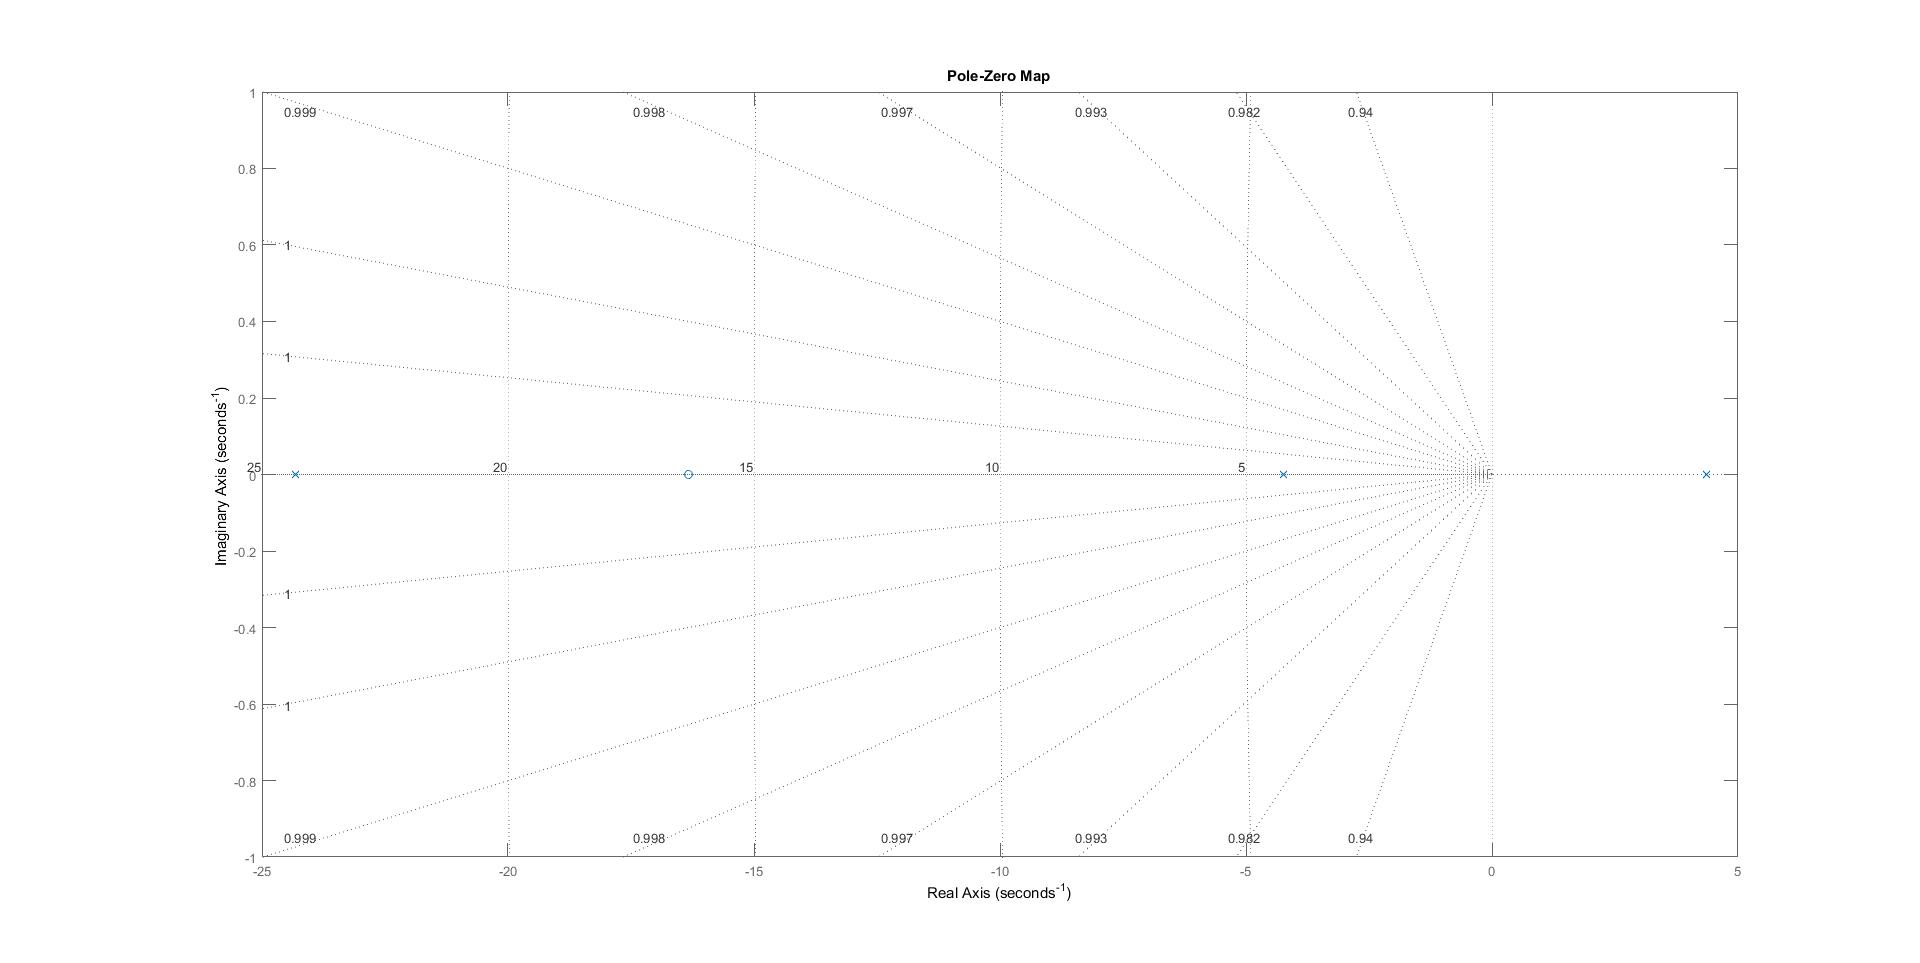
\includegraphics[height=10cm, width = 17cm]{h1fig.jpg}
\label{fig:pz1}
\centering
\end{figure}
\begin{figure}[h] 
\caption{Pole-Zero Plot of $H_2$ from \texttt{stability.m}}
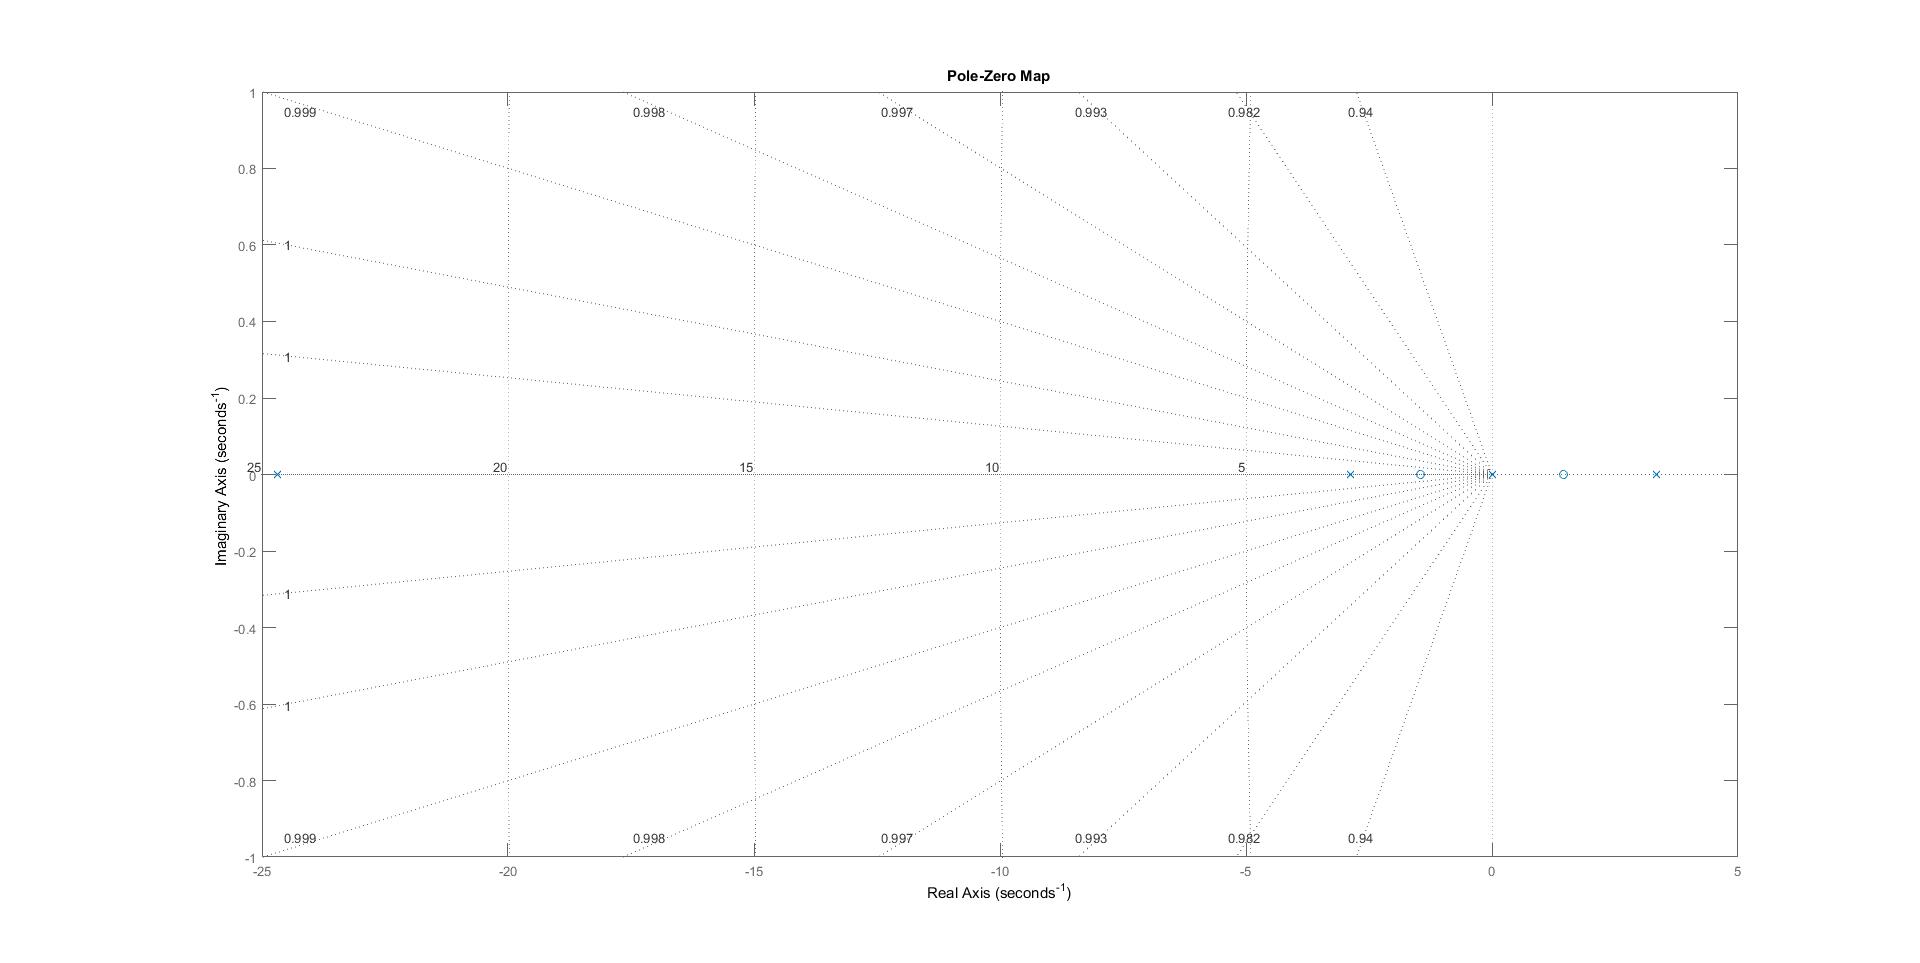
\includegraphics[height=10cm, width = 17cm]{h2fig.jpg}
\label{fig:pz2}
\centering
\end{figure}
\subsection{Equilibrium Points}
In order to find the equilibrium points of the open-loop linearized system the state space function in~\ref{eq:stateSpace} , are set to equal zero, when there is no voltage applied. Solving for the zero condition the following result is obtained: 
\begin{equation}
\begin{cases}
x_{1e}' = x_3 = 0 \\
x_{2e}' = x_4 = 0 \\
x_{3e}' = -2.8340x_2 - 24.2077x_3\\
x_{4e}' = 6.9760x_2 +24.2077x_3\\
\end{cases}
\end{equation}
From the above it can be seen that an equilibrium point exists when:
\begin{equation}
x_2,x_3,x_4 = 0 \; \; \; \; \forall x_1 \in \mathbb{R}
\end{equation}
\subsection{Controllability}
In order to determine the controllability of the controllability of the system the rank of the controllability matrix $\mathbb{C}$ must be determined and compared to the rank of the state space matrix $A$ state in equation~\ref{eq:stateSpace}. If $\mathbb{C}$ has a rank equal to $A$ then the system is controllable. 
\begin{equation}
\mathbb{C} = 
\begin{bmatrix}
B & AB & A^2B & A^3B \\
\end{bmatrix}
\end{equation}

\begin{equation}
\mathbb{C} = 
\begin{bmatrix}
0 & \frac{K_mK_g}{m_{cart}rR_A} & -\frac{K_m^2K_g^2}{m_{cart}^2r^3R_A^2} & \frac{K_m^5K_g^5}{m_{cart}^3r^5R_A^3}+\frac{K_mK_gmg}{m_{cart}^2lrR_A} \\
0 & -\frac{K_mK_g}{m_{cart}rR_A} & \frac{K_m^3K_g^3}{m_{cart}^2lr^3R_A^2} & -\frac{K_m^5K_g^5}{m_{cart}^3lr^5R_A^3}-\frac{g \Delta m K_mK_g}{m_{cart}^2l^2rR_A} \\
\frac{K_mK_g}{m_{cart}rR_A} & -\frac{K_m^3K_g^3}{m_{cart}^2r^3R_A^2} & \frac{K_m^5K_g^5}{m_{cart}^3r^5R_A^3}+\frac{mgK_mK_g}{m_{cart}^2lrR_A} & -\frac{K_m^7K_g^7}{m_{cart}^4r^7R_A^4} - \frac{mgK_m^3K_g^3}{m_{cart}^3lr^3R_A^2} - \frac{K_m^3K_g^3mg}{m_{cart}^3l^2r^3R_A^2} \\
-\frac{K_mK_g}{m_{cart}lrR_A} & -\frac{K_m^3K_g^3}{m_{cart}^2lr^3R_A^2} & -\frac{K_m^5K_g^5}{m_{cart}^3lr^5R_A^3}-\frac{g \Delta m K_mK_g}{m_{cart}^2l^2rR_A} & -\frac{K_m^7K_g^7}{m_{cart}^4r^7R_A^4} - \frac{K_m^7K_g^7}{m_{cart}^4l^2r^7R_A^4} + \frac{K_m^3K_g^3mg}{m_{cart}^3l^2r^3R_A^2} \\
\end{bmatrix}
\end{equation}


The controlabillity of this matrix was foun using \textit{MATLAB}.This was done by running simulations as row reduction would be too difficult.The \textit{MATLAB} output of \texttt{openLoopControllability.m} shows that the system is controllable. 
\subsection{Observability}
The observability matrix $\mathbb{O}$ is used in order to determine if the system is observable.  If the rank of $\mathbb{O}$ is equal to the rank of the state space matrix $A$, then the system is observable. 

\begin{equation}
\mathbb{O} = 
\begin{bmatrix}
C & CA & CA^2 & CA^3 \\
\end{bmatrix}^T
\end{equation}

\begin{equation} \label{eq:cont}
\mathbb{O} = 
\begin{bmatrix}
1 & 0 & 0 & 0 \\
0 & 1 & 0 & 0 \\
0 & 0 & 1 & 0 \\
0 & 0 & 0 & 1 \\
0 & -\frac{m_{ball}g}{m_{cart}} & -\frac{K_m^2K_g^2}{m_{cart}r^2R_A} & 0 \\
0 & \frac{g \Delta m}{m_{cart}l} & \frac{K_m^2K_g^2}{m_{cart}lr^2R_A} & 0 \\
0 & \frac{K_m^2K_g^2m_{ball}g}{m_{cart}^2r^2R_A} & \frac{K_m^4K_g^4}{m_{cart}^2r^4R_A^2} &  -\frac{m_{ball}g}{m_{cart}} \\
0 & -\frac{K_m^2K_g^2m_{ball}g}{m_{cart}^2lr^2R_A} & -\frac{K_m^4K_g^4}{m_{cart}^2lr^4R_A^2} & \frac{g \Delta m}{m_{cart}l} \\
\end{bmatrix}
\end{equation}
It can be seen that the matrix in ~\ref{eq:cont} has a rank of four by inspection. This can also be confirmed using the \textit{MATLAB} script   \texttt{openLoopObservability.m}. Therefore the open-loop system is observable.
\section{Linear Controllers}
The following section will discuss the design, simulation and analysis of controllers that can be used to stabilize the system in the upright position $\theta \approx 0^{\circ}$. The output variable that we are interested in controlling is $\theta$ and not $x$ as the linear position of the cart has complete freedom in this control problem. This is why the only transfer function of interest is $H_1(s)$ and the only time response of interest is $\theta(t)$.
\subsection{Pole-Placement}\label{sec:oneDOF}

The previous section ~\ref{sec:stability} showed that the open-loop state transfer function $H_1(s)$ is unstable because there exists a pole in the right- hand side of the $s$-plane. In the following section a one degree of freedom pole placement controller will be examined in order to control the closed loop system. 


In order to create a one degree of freedom (ODOF) pole placement controller the transfer function $H_1(s)$ must be modified using a feedback loop and design blocks in order to create a stable closed-loop transfer function. The figure ~\ref{fig:one_dof_block} represents the control system.
\begin{figure}[h] 
\caption{Block Diagram [3]}
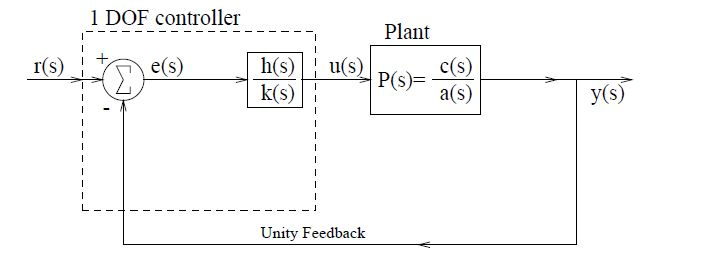
\includegraphics[height=5cm, width = 10cm]{./images/one_dof_block.jpg}
\label{fig:one_dof_block}
\centering
\end{figure}
In order to simplfy the problem, the design block $\frac{h(s)}{k(s)}$ is considered to be a proportionality constant, $K$, with no powers of $s$. This simplifies the analysis, yielding a closed-loop transfer function of:
\begin{equation}
T(s) = \frac{Kc(s)}{a(s) + Kc(s)}
\end{equation}In order to create the controller, the parameter $K$ must be edited. The script \texttt{poleplacement.m}prints the threshold value of k that make the system stable. The script also displays the poles with that $K$ value and the R-LocSus graph. The R-Locus graph shows how the poles will move as the value of $K$ changes. The R-Locus graph can be seen in figure ~\ref{fig:root} . Looking at the plot it shows that for many values of $K$ the system will remain unstable. But if $K$ gets large enough the system will become stable as no poles will be in the right hand plane. The correct value of k was tested for and it was found that its threshold value was: 
\begin{equation}
K \geq 1.48
\end{equation}
The stable pole-zero plot of the closed-loop system when $K = 1.48$ can be seen in figure ~\ref{fig:pz4}. 
\begin{figure}
\caption{RLocus}
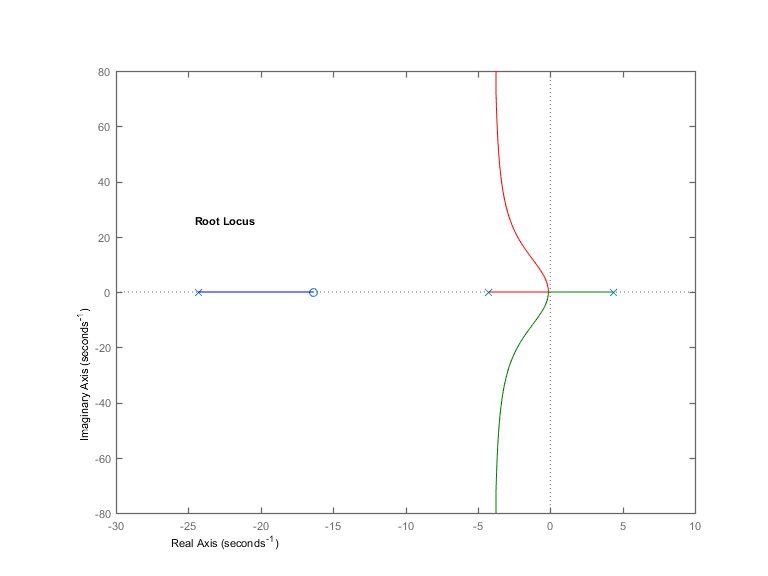
\includegraphics[height=9cm, width = 15cm]{polePlacementLotus.png}
\label{fig:root}
\centering
\end{figure}
\begin{figure}
\caption{Pole-Zero Pot of $T(s)$ when $K=1.48$}
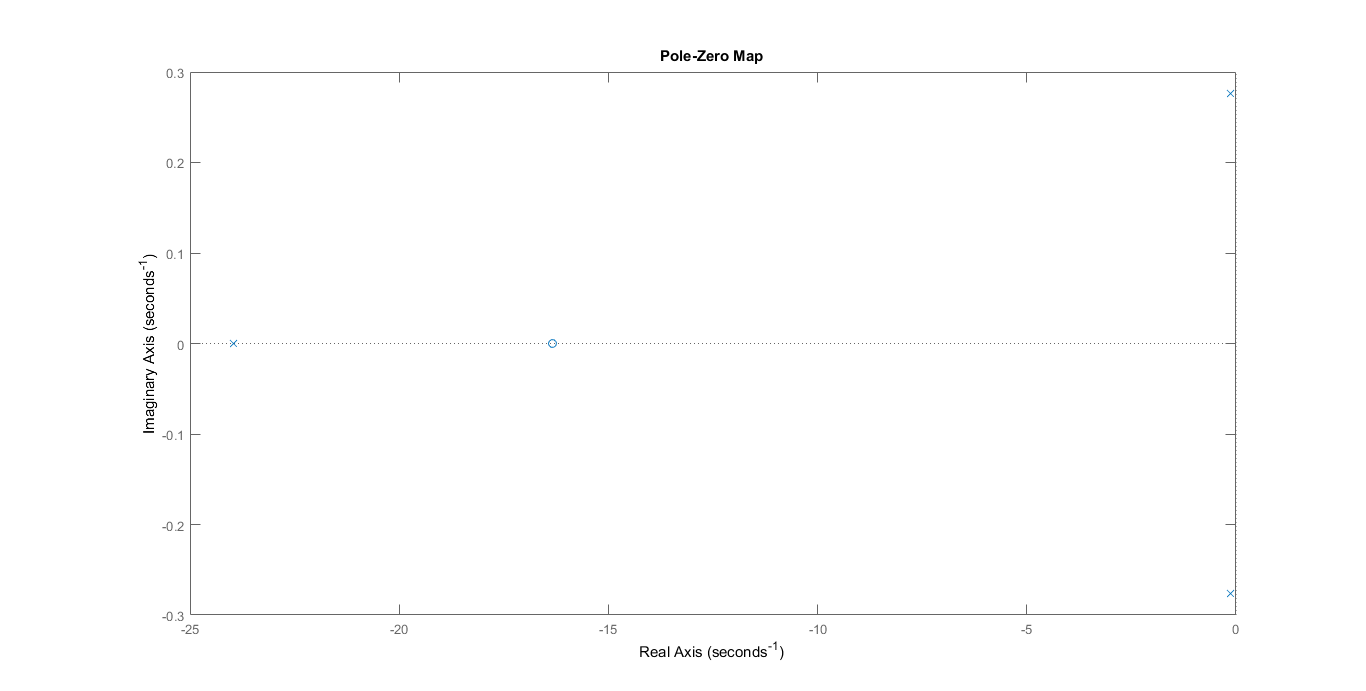
\includegraphics[height=10cm, width = 16cm]{poleplacementpoles.png}
\label{fig:pz4}
\centering
\end{figure}
\subsection{PID Controller}
The following section will describe the design and the analysis of a proportional-integral-derivative (PID) controller with a single degree of freedom. A PID controller calculates the mount of error between the desired point ($\theta \approx 0^{\circ}$) and the state ($\theta$). The controller attemps to minimize the error by changing the process based on the amount of error, the past error and the future error through a negative feedback action. The single degree of freedom controller discussed in the following section is implemented in the script \texttt{pidController.m}, which produces tuned output plots. A single degree PID system can be visualized in figure ~\ref{fig:PID_oneDOF}. 
\begin{figure}[h] 
\caption{PID One DOF Block Diagram [5]}
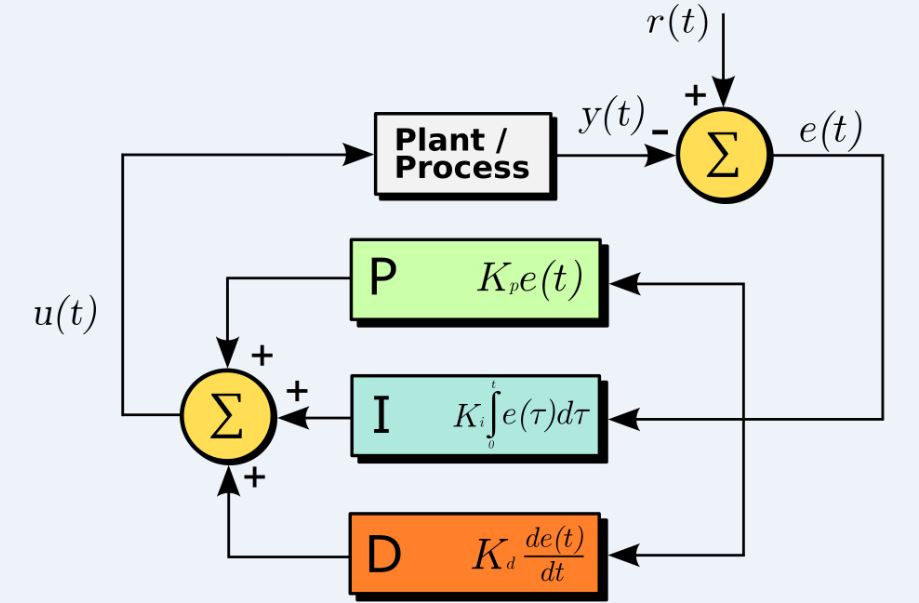
\includegraphics[height=6cm, width = 10cm]{./images/PID_oneDOF.jpg}
\label{fig:PID_oneDOF}
\centering
\end{figure}
This controller is similar to the single degree of freedom pole placement controller as only one design block is placed with the open-loop system. This one block is the only one that can be modified to achieve the stability desired. The block is the sum of three weighted error relations and is described mathematically in [3] in the following way: 
\begin{equation}
PID(s) = K_p + \frac{K_i}{s} + K_d s
\end{equation}
The terms $K_p, \;, K_i, \;K_d$ are the constants that are used in order to control the weights of the expression. Using the PID transfer function and placing it in a negative feedback loop with the open-loop transfer function $H(s)$ obtained earlier, produces the following closed-loop transfer function:
\begin{equation}
T(s) = \frac{H(s)}{1 + PID(s) H(s)} = \frac{c(s)}{a(s) + PID(s)c(s)}
\end{equation}
As the open-loop transfer function as found earlier has three poles and one zero , 
\begin{equation}
 H(s) = \frac{c(s)}{a(s)} = \frac{z_1s + z_0}{p_3s^3 + p_2s^2 + p_1s + p_0}
\end{equation}
Therefore the closed-loop transfer function is given by:
\begin{equation}
T(s) = \frac{z_1s^2 + z_0s}{p_3s^4 + (p_2+z_1K_d)s^3 + (p_1+z_1K_p+z_0K_d)s^2 + (p_0+z_1K_i+z_0K_p)s + (z_0K_i)}
\end{equation}

Now this controller must be tuned. This means that the weights of $K_p, \; K_i,$ and $K_d$ must be manipulated until a stable input response with a short settling time and a small deviation from the desired point of operation. At first $K_i,$ and $K_d$ where set to 0 and $K_p$ was set to the threshold value found in the previous section~\ref{sec:oneDOF}. The results where as expected creating a stable impulse response for $K_p \geq 1.48$. From this point the weights where gradually increased to improve the response. To increase the period of oscillations $K_p$ was increased. To reduce settling time $K_i$ was increased, and to reduce the peak deviation $K_d$ was increased [6]. Figure ~\ref{fig:impulse_tuned} shows the impulse response with the weight parameters tuned values.
 
\begin{figure}[h] 
\caption{Impulse Response of Tuned PID Controller $K_p = 250, K_i = 5, K_d = 30$}
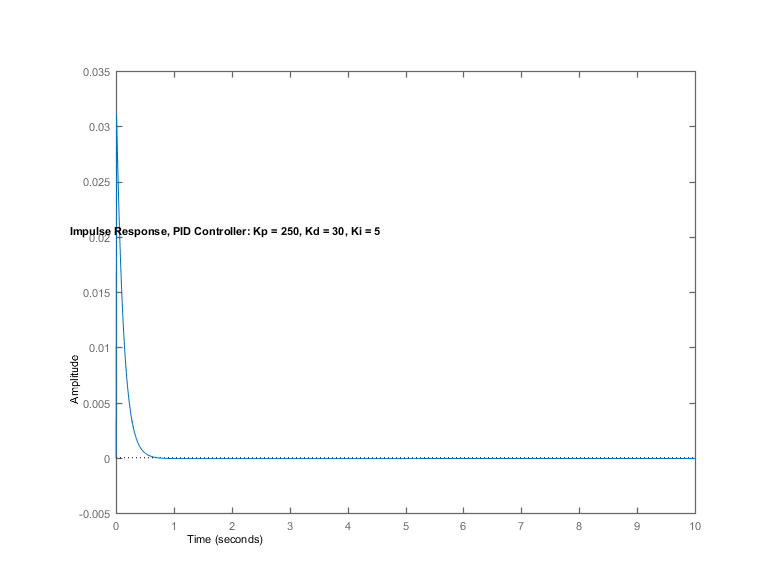
\includegraphics[height=8cm, width = 10cm]{impulsePID.png}
\label{fig:impulse_tuned}
\centering
\end{figure}
The parameter values that were chosen are $K_p = 250, K_i = 5, K_d = 30$. These values produced a stable controller with settling time close to $.717$ a deviation from the desired value of about $.031$ radians.

\subsection{LQR Controller}

A linear quadratic regulator controller is a controller that has a full state feedback system. This allows for the stabilization of the unstable open-loop system. This means that the unstable system transfer function $H_1(s)$ can be stabilized. If the system was not observable it would not have been possible to implement the LQR controller for the stabilization of the system.
\\\\
\begin{figure}[h]
\caption{LQR Controller Block Diagram [7]}
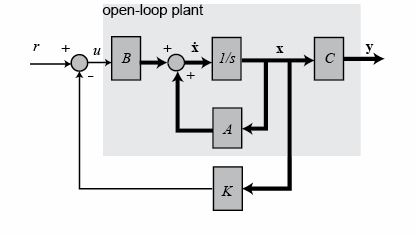
\includegraphics[height=5cm, width=8cm]{./images/lqr_block.jpg}
\label{fig:lqrblock}
\centering
\end{figure}

An LQR controller is used to determine the values of a system’s weight parameter on the linear and angular position $Q$ against the amount of error that is allowed in the system $R$ [7]. When these weights are decided the controller can compute the values for the gain matrix $K$. The gain matrix is then used to compute a new state space model where the $A$ matrix is altered through the subtraction by the $B$ matrix multiplied by $K$. The $B$, $C$ and $D$ matrices remain the same. 
\\\\
In \textit{MATLAB} the \texttt{lqr} function can be used for this process. As recommended by [6], the easiest way to begin picking values for $R$ and $Q$ is to start by assigning $R$ a value of one. These values are arbitrary and what is actually important is the ratio seen between $Q$ and $R$. This ratio will determine the weight of importance put on position and allowable error. Seeing as this project does not stress to much importance on the linear position, the weight of this was lowered in order to account for more accuracy elsewhere. This value is seen at the $(1,1)$ position of the $Q$ matrix. The $(2,2)$ position of the $Q$ matrix, which pertains to angular position importance, was raised substantially in order to obtain a better balancing system. The step response of the system utilizing the LQR controller and the system not utilizing it can be seen below in figures ~\ref{fig:lqrresult1} and ~\ref{fig:lqrresult2}. As can be seen, the fluctuation in angular and linear position decreases heavily as the values of Q have been raised, showing that this is overall a very effective, balancing controller. The \textit{MATLAB} implementation of the LQR controller discussed here can be found in \texttt{InvertedPend\_LQR.m}.
\FloatBarrier
\begin{figure}[h]
\caption{Unstable Open-Loop Step Response without LQR}
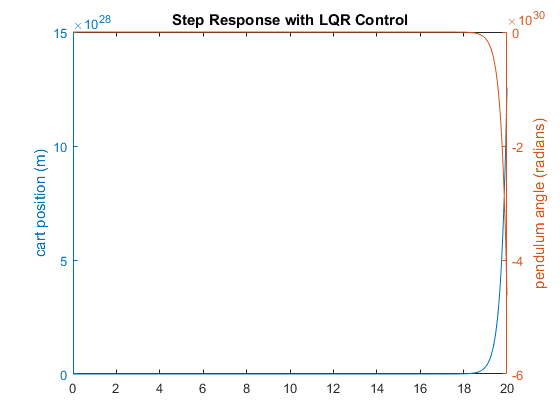
\includegraphics[height=8cm, width=10cm]{LQRno.png}
\label{fig:lqrresult1}
\centering
\end{figure}
\begin{figure}[h]
\caption{Stable Closed-Loop Step Response with low ratio LQR}
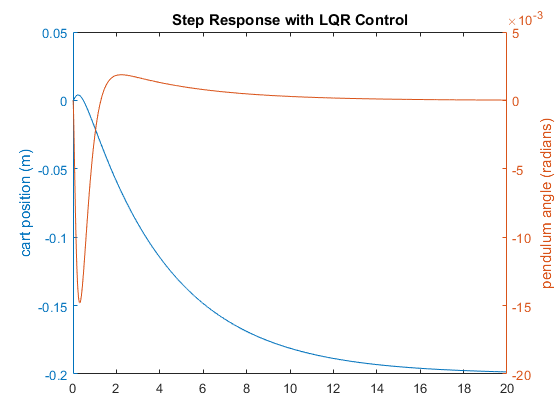
\includegraphics[height=8cm, width=10cm]{LQR11.png}
\label{fig:lqrresult2}
\centering
\end{figure}
\FloatBarrier
\begin{figure}[h]
\caption{Unstable Open-Loop Step Response high ratio LQR}
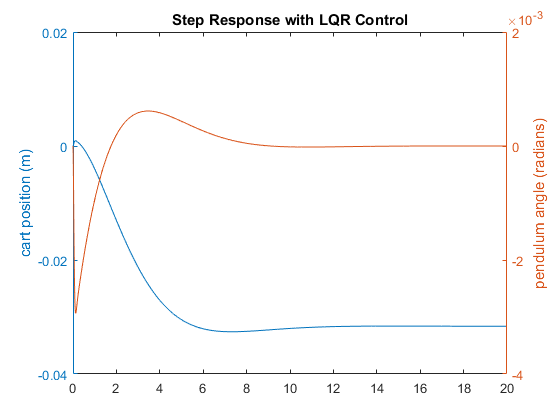
\includegraphics[height=8cm, width=10cm]{LQR404000.png}
\label{fig:lqrresult1}
\centering
\end{figure}
\subsection{Discussion of Results}
One of the controllers must be chosen in order to stabilize the system. There are several advantages and disadvantages to the controllers. The properties that will help guide which one should be chosen are stability, gain margin, phase margin, settling time, max deviation from set-point, and practicality. The best performance comes from the PID and LQR controllers which have short settling times and small deviations from the desired operating point. 

\subsection{Stabilization Neighborhood} \label{sec:neigh}
\section{Conclusion}
The inverted pendulum control problem can be stabilized using various controllers. Each controller has its trade-offs and advantages. The most challenging aspect of the design is fine tuning the parameters of the controllers in order to obtain good stabilizations. It was concluded that the best controllers where the LQR and PID controllers as they could provide stabilization in different circumstances with little time and little deviation from the desired point. Though the PID is concluded to be better as it transitions well with the non-linear model.   
\newpage

\section{Works Cited}
\begin{itemize}
\item [[$\;$ 1]] Michalska, H., ECSE 404: 304-404 section 1. 
Obtained from McGill University MyCourses. Fall 2014
\item [[$\;$ 2]] Technische Universität München, School of Computational Engineering., Pendulum Project [Online]. Available: http://www5.in.tum.de/wiki/index.php/Pendulum \_Project
\item [[$\;$ 3]] Michalska, H., ECSE 404: 304-404 section 6. 
Obtained from McGill University MyCourses. Fall 2014
\item [[$\;$ 4]] Michalska, H., ECSE 404: 304-404 section 7. 
Obtained from McGill University MyCourses. Fall 2014
\item [[$\;$ 5]] Wikipedia., PID Controller [Online]. Available: 
en.wikipedia.org/wiki/PID\_controller
\item [[$\;$ 6]] University of Michigan, School of Engineering., Extras: Designing Lead and Lag Compensators [Online]. Available: http://ctms.engin.umich.edu/CTMS/index.php? aux=Extras\_Leadlag
\item [[$\;$ 7]]  University of Michigan, School of Engineering., Inverted Pendulum: State-Space Methods for Controller Design [Online]. Available: http://ctms.engin.umich.edu/ CTMS/index.php?example=InvertedPendulum\&section=ControlStateSpace
\end{itemize}
\end{document}